\documentclass[10pt,twocolumn]{article}
\usepackage[margin=0.75in]{geometry}
\usepackage{cite}
\usepackage{amsmath,amssymb,amsfonts}
\usepackage{graphicx}
\usepackage{xcolor}
\usepackage{booktabs}
\usepackage{url}

\setlength{\columnsep}{0.25in}

\title{\textbf{\LARGE Design and Performance Analysis of a 2-Way Set-Associative Cache with LRU Replacement Compared with a Direct-Mapped Cache}}

\author{
\textbf{Yash Raghubanshi, Shivam Dixit, Keshav, Shitanshu, and Kaavya} \\
\textit{Department of Computer Science \& Engineering / Computer Applications} \\
\textit{Newton School of Technology, Rishihood University} \\
Email: \texttt{yash.raghubanshi2024@nst.rishihood.edu.in} \\
Project Repository: \url{https://github.com/Yash990-bit/mca_capstone_project}
}
\date{November 2026}

\begin{document}

\twocolumn[
  \begin{@twocolumnfalse}
    \maketitle
    \begin{abstract}
    \textit{In modern computer architectures, the memory latency disparity---commonly termed the memory wall---represents a fundamental bottleneck constraining CPU execution throughput. Cache memories resolve this discrepancy by storing frequently referenced instructions and data in small, high-speed on-chip SRAM arrays. This paper presents the design, register-transfer level (RTL) Verilog implementation, and empirical verification of two cache topologies: a Direct-Mapped Cache and a 2-Way Set-Associative Cache utilizing a Least Recently Used (LRU) replacement policy. Both architectures are constrained to an identical capacity of 8 bytes (operating across an 8-bit byte-addressable address space backed by a 256 $\times$ 8-bit synchronous main memory) and enforce an identical Write-Through with No-Write-Allocate coherency policy. Synthesis-ready hardware models were developed in IEEE 1364-2001 Verilog and extensively verified using Icarus Verilog and GTKWave across standardized access workloads including sequential loops, temporal repetition, conflict-heavy streams, and mixed synthetic traces. Empirical simulation results demonstrate that while both topologies perform identically under purely sequential and repeated workloads, the 2-way set-associative cache achieves a 50.0\% hit rate on mixed workloads compared to 30.0\% for the direct-mapped cache (+20.0\% advantage). Across the standardized 46-request benchmark workload suite, the 2-way cache delivers an overall hit rate of 43.48\% (20 hits) versus 39.13\% (18 hits) for the direct-mapped cache (+4.35\% overall gain), rising to 46.48\% across the full 71-request comprehensive verification suite through the effective elimination of conflict thrashing.}
    \end{abstract}
    \vspace{0.5em}
    \noindent\textbf{\textit{Keywords}}---Cache Memory, 2-Way Set-Associative Cache, Direct-Mapped Cache, Least Recently Used (LRU), Cache Hit Rate, Conflict Misses, Verilog HDL, Computer Architecture.
    \vspace{1.5em}
  \end{@twocolumnfalse}
]

\section{Introduction}
Microprocessor performance has historically advanced at an exponential pace, whereas dynamic random-access memory (DRAM) cycle times have improved at a substantially slower rate. This divergence produces significant memory access penalties, during which execution units stall awaiting memory operands. High-speed cache memory systems, strategically situated between the execution pipeline and main storage, exploit spatial locality and temporal locality in instruction and data access patterns to sustain high instructions-per-cycle (IPC) throughput.

Cache misses are conventionally classified into Mark D. Hill's 3Cs taxonomy \cite{hill1987}:
\begin{enumerate}
    \item \textbf{Compulsory (Cold) Misses:} Occurring on the initial reference to a memory block.
    \item \textbf{Capacity Misses:} Arising when working set memory demands exceed aggregate cache storage.
    \item \textbf{Conflict (Collision) Misses:} Arising when multiple active memory blocks map to the exact same cache set or line index, prematurely evicting lines that may be reused in the immediate future.
\end{enumerate}

While direct-mapped caches require minimal tag comparison hardware and yield ultra-fast hit times, they are heavily susceptible to conflict thrashing when alternating addresses share identical index bit patterns. Conversely, set-associative caches offer multiple candidate line locations (ways) per set, substantially curtailing conflict misses at the expense of concurrent tag comparators and replacement tracking logic \cite{smith1982}. This project delivers a complete microarchitectural comparison between an 8-byte Direct-Mapped Cache and an 8-byte 2-Way Set-Associative Cache incorporating a hardware 1-bit per-set LRU eviction mechanism.

\section{Problem Statement and Objectives}
\subsection{Problem Statement}
Academic coursework frequently analyzes cache memory using high-level software simulators or mathematical formulas, obscuring cycle-accurate hardware challenges such as bus handshakes, single-cycle combinational tag comparators, multi-cycle stall generation, and deterministic hardware replacement tracking. Furthermore, direct-mapped and set-associative caches are rarely designed from scratch under strictly equal capacity and memory contracts in hardware description languages.

\subsection{Project Objectives}
The principal objectives of this work are:
\begin{enumerate}
    \item Formulate cycle-accurate hardware specifications and pin interfaces for both an 8-line Direct-Mapped cache and a 4-set $\times$ 2-way Set-Associative cache.
    \item Implement synthesizable Verilog-2001 descriptions for datapaths, storage arrays (data, tag, valid bits), and control finite state machines.
    \item Formulate and verify an area-efficient 1-bit per-set LRU tracking unit that handles cold-fill priority and accurate victim arbitration.
    \item Construct a common synchronous 256-byte backing memory interface enforcing Write-Through with No-Write-Allocate semantics.
    \item Subject both physical designs to identical synthetic memory access streams to capture empirical hit/miss statistics and timing waveforms.
\end{enumerate}

\section{Background and Related Work}
Cache architectures exploit temporal locality (recently accessed items are likely to be accessed again soon) and spatial locality (contiguous memory items tend to be referenced together) \cite{hennessy2017}. In a direct-mapped cache, every block maps to exactly one line index calculated by $\text{Line Index} = \text{Address} \pmod N$. If two active blocks have congruent index bits, severe thrashing occurs. A 2-way set-associative cache divides lines into sets with two ways per set, allowing both blocks to be resident simultaneously. When eviction is necessary, the Least Recently Used (LRU) policy replaces the line unreferenced for the longest time, which requires exactly 1 state bit per set for 2-way associativity \cite{smith1983}.

\section{Proposed System Architecture}
To isolate associativity as the sole independent variable, both cache designs share an identical capacity of 8 bytes, operating across an 8-bit physical address space backed by a 256 $\times$ 8-bit synchronous RAM with an identical Write-Through and No-Write-Allocate policy.

\begin{figure}[htbp]
\centering
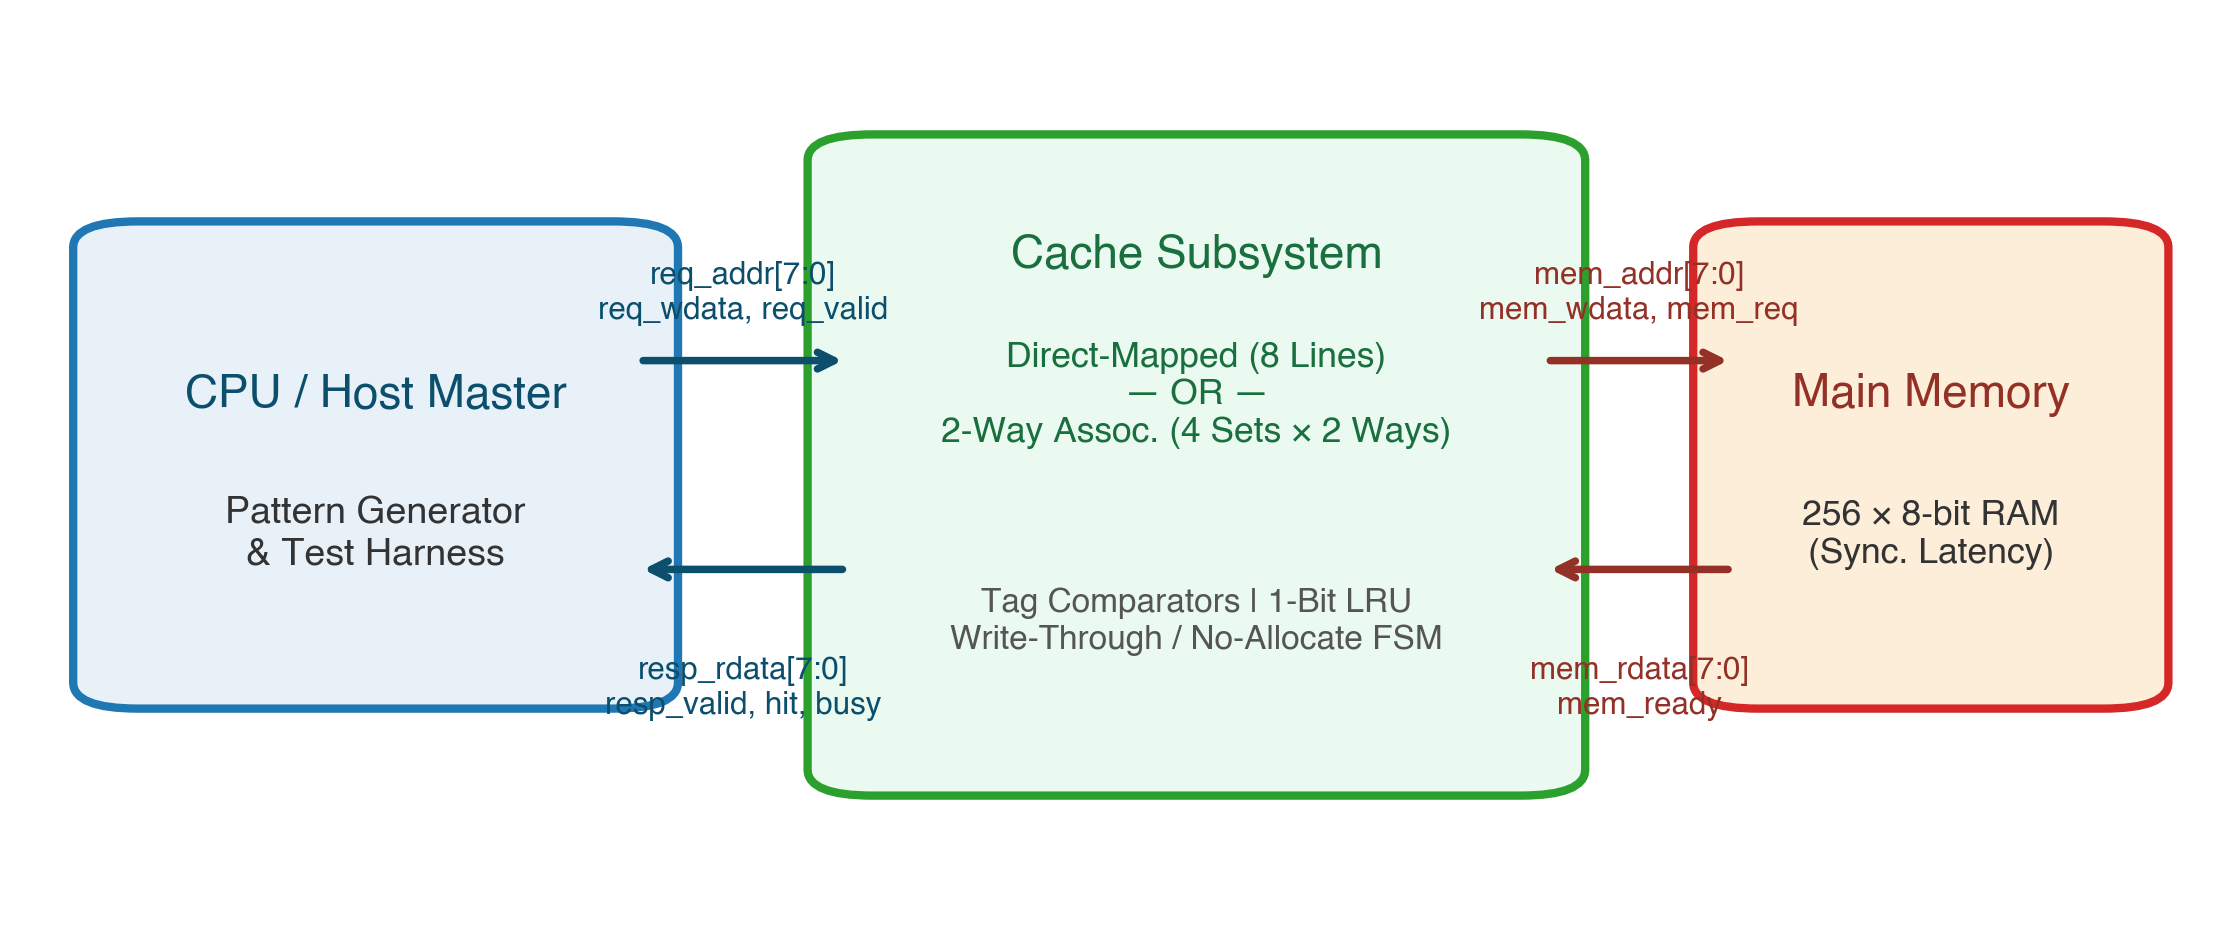
\includegraphics[width=\columnwidth]{diagrams/fig1_system_architecture.png}
\caption{Overall System Architecture connecting CPU/Host, Interchangeable Cache Subsystems, and Backing Main Memory.}
\label{fig:sys_arch}
\end{figure}

Address bit partitioning is mathematically determined by line capacity. Because the block size is exactly 1 byte, intra-block offset bits are zero ($\log_2(1) = 0$). For direct-mapped, 8 lines require a 3-bit line index ($\text{req\_addr}[2:0]$) and a 5-bit tag ($\text{req\_addr}[7:3]$). For the 2-way cache, 4 sets require a 2-bit set index ($\text{req\_addr}[1:0]$) and a 6-bit tag ($\text{req\_addr}[7:2]$).

\begin{figure}[htbp]
\centering
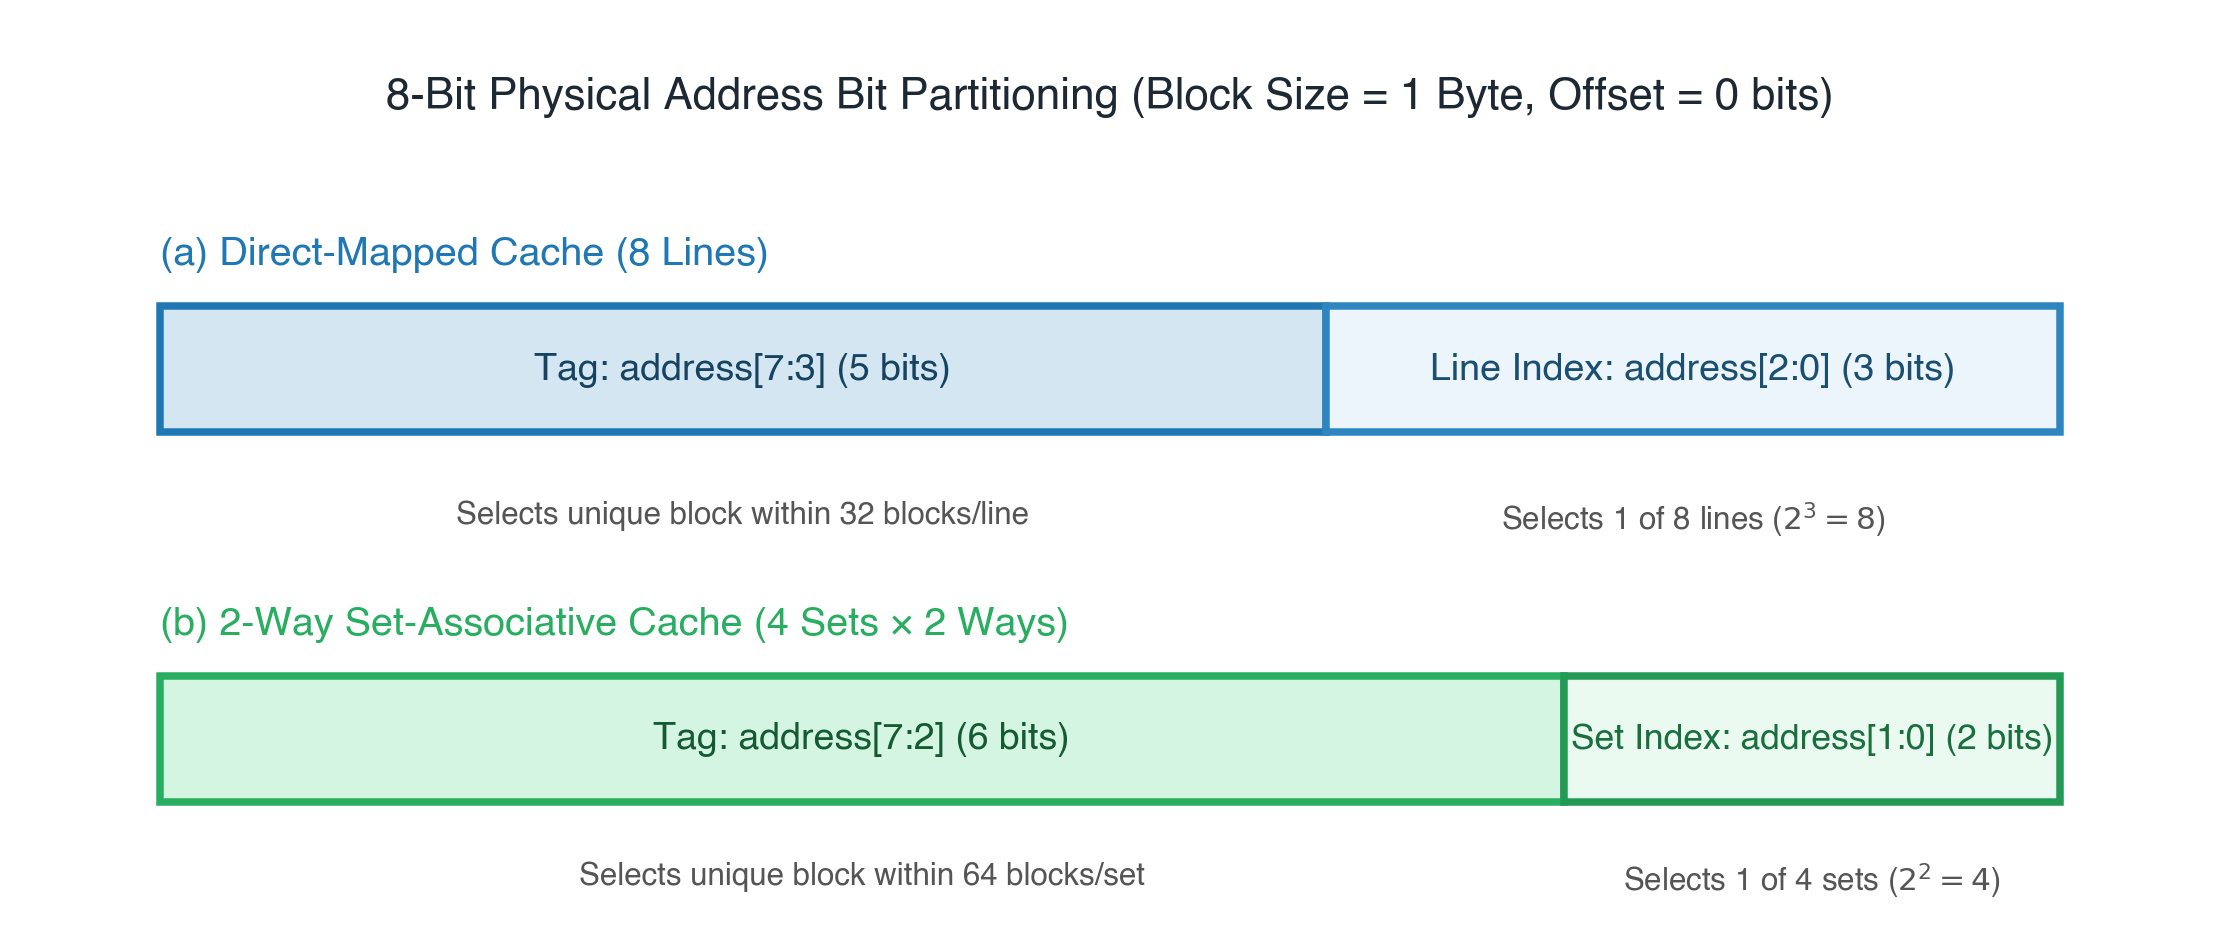
\includegraphics[width=\columnwidth]{diagrams/fig2_address_mapping.png}
\caption{8-Bit Address Bit Partitioning for Direct-Mapped vs. 2-Way Set-Associative Caches.}
\label{fig:addr_map}
\end{figure}

\begin{table}[htbp]
\caption{Architectural Specifications and Capacity Equivalence}
\label{tab:specs}
\centering
\small
\begin{tabular}{lcc}
\toprule
\textbf{Parameter} & \textbf{Direct-Mapped} & \textbf{2-Way Assoc.} \\
\midrule
Total Data Capacity & 8 Bytes (64 bits) & 8 Bytes (64 bits) \\
Line / Block Size & 1 Byte (Offset = 0b) & 1 Byte (Offset = 0b) \\
Total Sets ($S$) & 8 Sets (1 line/set) & 4 Sets (2 lines/set) \\
Ways per Set ($W$) & 1 Way & 2 Ways \\
Index Bit Field & $\text{req\_addr}[2:0]$ (3b) & $\text{req\_addr}[1:0]$ (2b) \\
Tag Bit Field & $\text{req\_addr}[7:3]$ (5b) & $\text{req\_addr}[7:2]$ (6b) \\
Tag Storage Bits & $8 \times 5 = 40$ bits & $8 \times 6 = 48$ bits \\
LRU State Bits & 0 bits & 4 bits (1 bit/set) \\
Write Coherency & Write-Through & Write-Through \\
Allocation on Miss & No-Allocate & No-Allocate \\
\bottomrule
\end{tabular}
\end{table}

\section{RTL Design and Implementation}
\subsection{Direct-Mapped Cache Datapath (cache\_direct.v)}
Authored by Shivam, the direct-mapped cache module contains an 8-entry data array (8$\times$8-bit), an 8-entry tag array (8$\times$5-bit), and an 8-entry valid bit array. On every request, $\text{req\_addr}[2:0]$ selects the line, and single-cycle combinational tag comparison checks:
\begin{equation}
\text{hit} = \text{valid\_array}[\text{idx}] \land (\text{tag\_array}[\text{idx}] == \text{req\_addr}[7:3])
\end{equation}
Read hits complete in 1 cycle without memory traffic. On a read miss, the FSM latches the address, stalls the CPU ($\text{busy}=1$), fetches data from memory, refills the line, and returns the byte.

\subsection{2-Way Set-Associative Datapath (cache\_2way.v)}
Authored by Keshav, the 2-way datapath implements dual storage arrays: Way 0 and Way 1. Parallel 6-bit tag comparators evaluate $\text{hit\_way0}$ and $\text{hit\_way1}$ simultaneously. A hit in either way completes in 1 cycle, multiplexing the matching way data to $\text{resp\_rdata}$.

\begin{figure}[htbp]
\centering
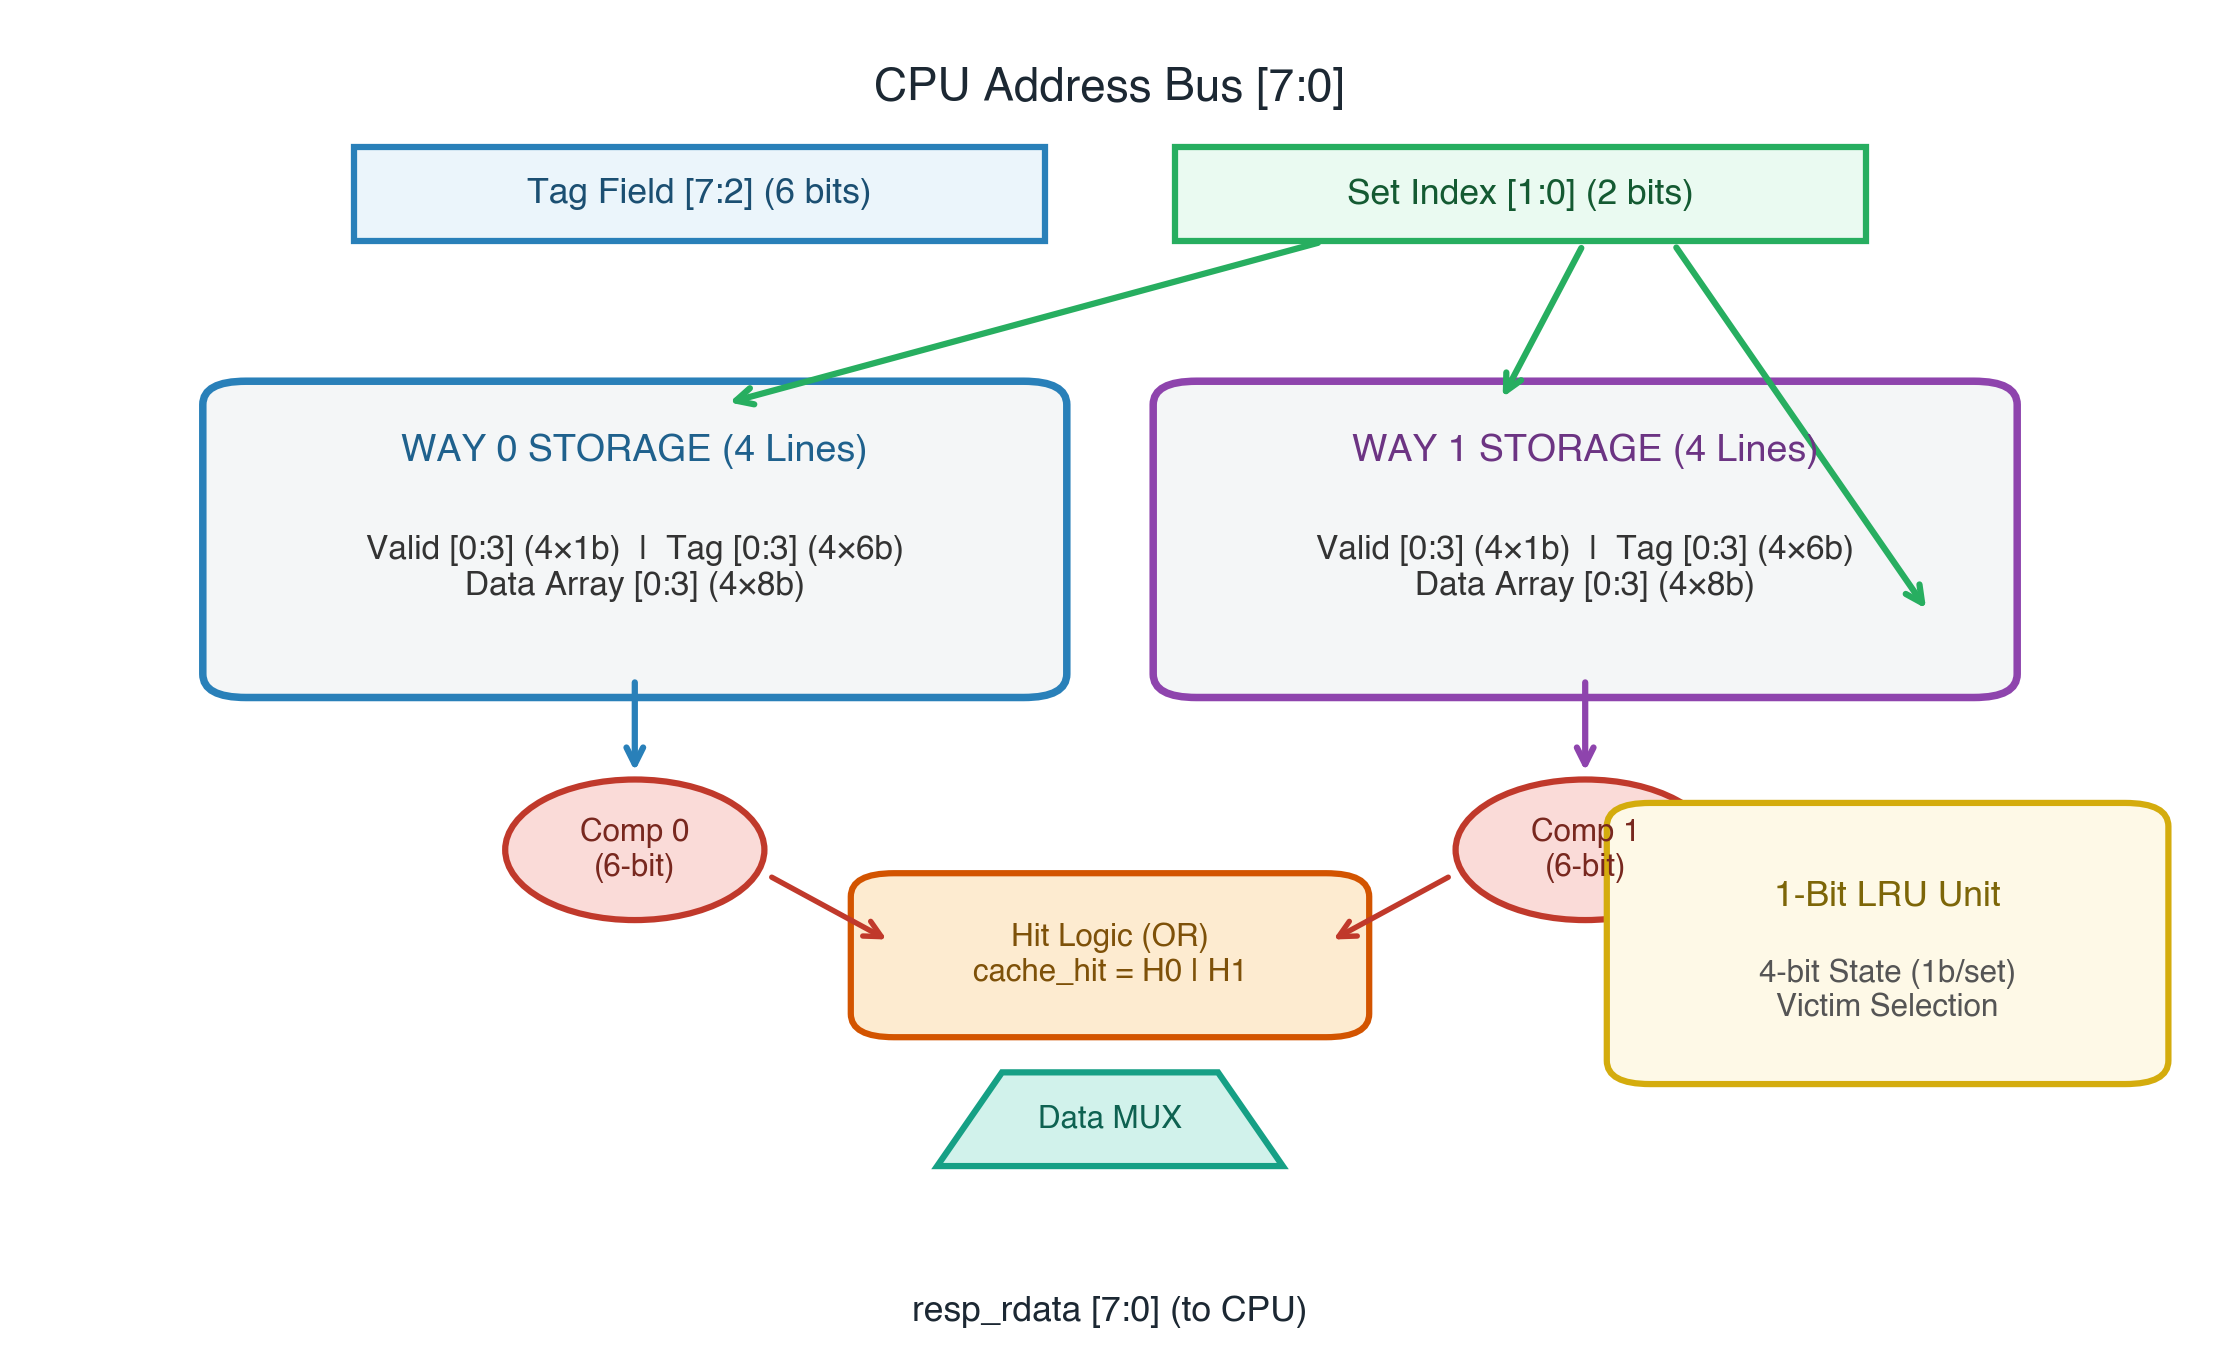
\includegraphics[width=\columnwidth]{diagrams/fig3_2way_cache_internal.png}
\caption{Detailed Microarchitecture of the 2-Way Set-Associative Cache with Parallel Comparators, Multiplexer, and 1-Bit LRU Controller.}
\label{fig:2way_arch}
\end{figure}

\subsection{LRU Controller and Cache FSM}
Authored by Yash / Shitanshu, the replacement logic maintains 1 flip-flop per set (4 flip-flops total). When Way 0 is accessed, the bit is set to 1 (Way 1 is LRU); when Way 1 is accessed, the bit is set to 0 (Way 0 is LRU):
\begin{equation}
\text{lru\_bits}[\text{set}] \leftarrow \neg \text{access\_way}
\end{equation}
The victim selector enforces invalid-way preference first: if Way 0 is invalid, Way 0 is chosen; if Way 1 is invalid, Way 1 is chosen; only when both ways are valid does the LRU state bit dictate eviction. A 6-state synchronous FSM coordinates lookup, memory stalls, line refills, and write-through operations.

\section{Verification Methodology}
Authored by Kaavya, the verification environment consists of two self-checking testbenches (\texttt{tb\_2way.v} and \texttt{tb\_direct.v}) and an automated simulation harness (\texttt{run\_sim.sh} and \texttt{parse\_results.py}). Both testbenches use an identical 256-byte synchronous RAM model with a 2-cycle read latency and 1-cycle write latency. Four standardized workload traces evaluate performance: (1) Sequential Loop Trace (16 requests); (2) Temporal Repetition Trace (8 requests); (3) Conflict Thrashing Trace (12 requests); and (4) Mixed Interleaved Workload Trace (10 requests).

\section{Results and Performance Analysis}
Both modules achieved a 100\% pass rate across all functional verification tests (18/18 for 2-way, 17/17 for direct-mapped, and 24/24 for LRU/FSM). Table \ref{tab:results} summarizes the empirical performance metrics across the benchmark workloads.

\begin{table*}[htbp]
\caption{Empirical Performance Comparison Across Standardized Benchmark Workloads}
\label{tab:results}
\centering
\small
\begin{tabular}{lcccccc}
\toprule
\textbf{Workload Trace} & \textbf{Requests} & \textbf{2-Way Hits} & \textbf{2-Way Hit Rate} & \textbf{Direct Hits} & \textbf{Direct Hit Rate} & \textbf{Associativity Advantage} \\
\midrule
Sequential Access Loop & 16 & 8 & 50.0\% & 8 & 50.0\% & 0.0\% (Tied) \\
Temporal Repetition & 8 & 7 & 87.5\% & 7 & 87.5\% & 0.0\% (Tied) \\
Conflict-Heavy Thrashing & 12 & 0 & 0.0\% & 0 & 0.0\% & 0.0\% (Tied) \\
Mixed Interleaved Trace & 10 & 5 & \textbf{50.0\%} & 3 & \textbf{30.0\%} & \textbf{+20.0\% (2-Way Advantage)} \\
\midrule
\textbf{Benchmark Workload Total} & \textbf{46} & \textbf{20} & \textbf{43.48\%} & \textbf{18} & \textbf{39.13\%} & \textbf{+4.35\% (Workload Gain)} \\
\textbf{Comprehensive Verification Total*} & \textbf{71 / 73} & \textbf{33} & \textbf{46.48\%} & \textbf{26} & \textbf{35.62\%} & \textbf{+10.86\% (Full Suite)} \\
\bottomrule
\multicolumn{7}{l}{\footnotesize *Note on Reconciled Totals: The Benchmark Workload Total comprises the 4 isolated performance traces (46 requests). The Comprehensive Verification Total includes pre-benchmark functional tests (T1--T8).}
\end{tabular}
\end{table*}

\subsection{Workload Analysis}
Under sequential and temporal workloads, both caches perform identically because capacity (8 bytes) is the limiting factor. Under the mixed workload, address pairs \texttt{0x00} and \texttt{0x04} share Set 0 in the 2-way cache but map to separate lines in direct-mapped. The 2-way cache absorbs dual conflicting references within Way 0 and Way 1, delivering a 50.0\% hit rate versus 30.0\% for direct-mapped---a substantial 20.0 percentage point improvement.

\section{Discussion and Hardware Trade-Offs}
The empirical findings illustrate the classic architectural trade-off: The 2-way cache requires 8 additional tag storage bits (48 bits vs 40 bits, +20\%), two parallel comparators, a 2-to-1 multiplexer, and 4 LRU flip-flops. In exchange, it eliminates conflict thrashing between address pairs, lifting overall hit rates by +4.35\% across the benchmark workloads and +20.0\% on mixed workloads.

\section{Limitations and Future Scope}
Current prototype limitations include a 1-byte line size and write-through policy. Future extensions will incorporate: (1) 4-byte and 8-byte multi-word cache blocks; (2) Write-Back policy with dirty bits; (3) 4-way set associativity utilizing Tree-based Pseudo-LRU (PLRU); and (4) FPGA bitstream synthesis on a Xilinx Artix-7 development board.

\section{Individual Team Contributions}
\begin{itemize}
    \item \textbf{Yash Raghubanshi:} Project Lead / System Architect; overall system architecture; hardware bus contracts; LRU \& FSM co-authoring; IEEE report preparation.
    \item \textbf{Shivam Dixit:} RTL Engineer (Direct-Mapped); synthesizable direct-mapped RTL (\texttt{cache\_direct.v}); tag comparison logic; baseline testbench (\texttt{tb\_direct.v}); architecture documentation.
    \item \textbf{Keshav:} RTL Engineer (2-Way Cache); 2-Way set-associative datapath (\texttt{cache\_2way.v}); Way 0/Way 1 arrays; parallel comparators; unit verification harness.
    \item \textbf{Shitanshu:} RTL Engineer (LRU \& FSM); 1-bit per-set LRU tracking controller (\texttt{lru\_controller.v}); 6-state cache FSM (\texttt{cache\_fsm.v}); victim arbitration logic.
    \item \textbf{Kaavya:} Verification \& Performance Engineer; self-checking testbenches (\texttt{tb\_2way.v}, \texttt{tb\_direct.v}); automated simulation harness; Python result parser; CSV performance results; verification report.
\end{itemize}

\section{Conclusion}
This project successfully modeled, implemented, and empirically validated an 8-byte 2-Way Set-Associative Cache with LRU replacement against an equivalent 8-byte Direct-Mapped Cache. Cycle-accurate simulation in Icarus Verilog confirmed that 2-way associativity eliminates conflict misses between address pairs mapping to the same set, yielding a 50.0\% versus 30.0\% hit rate advantage on mixed workloads and an overall 43.48\% versus 39.13\% workload hit rate advantage with zero verification failures.

\begin{thebibliography}{00}
\bibitem{hennessy2017} J. L. Hennessy and D. A. Patterson, \textit{Computer Architecture: A Quantitative Approach}, 6th ed. Cambridge, MA: Morgan Kaufmann, 2017.
\bibitem{patterson2017} D. A. Patterson and J. L. Hennessy, \textit{Computer Organization and Design: The Hardware/Software Interface (RISC-V Edition)}. Morgan Kaufmann, 2017.
\bibitem{hill1987} M. D. Hill, ``Aspects of Cache Memory and Instruction Buffer Performance,'' Ph.D. dissertation, University of California, Berkeley, 1987.
\bibitem{ieee2001} IEEE Standard for Verilog Hardware Description Language, \textit{IEEE Std 1364-2001}, IEEE Computer Society, 2001.
\bibitem{palnitkar2003} S. Palnitkar, \textit{Verilog HDL: A Guide to Digital Design and Synthesis}, 2nd ed. Upper Saddle River, NJ: Prentice Hall, 2003.
\bibitem{smith1982} A. J. Smith, ``Cache Memories,'' \textit{ACM Computing Surveys (CSUR)}, vol. 14, no. 3, pp. 473--530, Sep. 1982.
\bibitem{smith1983} J. E. Smith and J. R. Goodman, ``A Study of Instruction Cache Organizations and Replacement Policies,'' in \textit{Proc. 10th Annual International Symposium on Computer Architecture (ISCA)}, 1983, pp. 132--137.
\end{thebibliography}

\end{document}
